\newpage
\thispagestyle{sectioned}
\chapter{Tecnologías del Proyecto}

En las siguientes secciones se explicarán brevemente las tecnologías y herramientas que se han utilizado para llevar a cabo este proyecto. Concretamente se hablará de las tecnologías utilizadas durante la Migración del cliente web de SwellRT (Wave) a Android (Ver Sección \ref{sec:migration}) y durante el desarrollo de la aplicación Android que hará uso del resultado de dicha Migración. 

En el caso de Wave, al tratarse de una tecnología bastante reciente, se explicará más detalladamente en qué consite esta tecnología, pero para el resto de casos se hará una pequeña reseña sobre en qué consiste la tecnología y sus usos. En todos los casos se intentará tambíen explicar de qué manera y para qué se ha utilizado dentro de este proyecto.

Para hacerse una idea general de las tecnologías utilizadas se recomienda ver el resumen que se muestra en la Tabla \ref{fig:technologiesTable}. 

	\begin{figure}[H]
	  \centering
	    \includegraphics[keepaspectratio, scale=0.2]{Media/Diagrams/technologies.png}
	  \caption{Nube de Tecnologías utilizadas en el Proyecto}
	  \label{fig:technologies}
	\end{figure}	
 
      \begin{table}[H]
	\footnotesize
	\begin{center}
	\begin{tabular}{| c | c | m{9cm} | c |}
	  \hline
	  \textbf{Tipo} & \textbf{Nombre} & \textbf{Uso} & \textbf{Sección} \\
	  \hline
	  \multirow{4}{*}{Framework} & SwellRT &  Framework que permite desarrollar aplicaciones con la tecnología y la infraestructura federada de Wave a través de un API JavaScript y Android. & \ref{sssec:swellRT} \\ \cline{2-4} 
	  & Android & Plataforma para la Migración y el Desarrollo de la app. & \ref{ssec:android} \\ \cline{2-4}
	  & GWT & Framework JavaScript utilizado por el antiguo Cliente web de Wave presente en SwellRT. & \ref{ssec:gwt} \\ \cline{2-4}
	  & Laravel 5 & Framework de desarrollo del Service REST de la App en PHP. & \ref{ssec:laravel} \\ \hline
	  \multirow{2}{*}{Servidor} & \begin{tabular}[c]{@{}c@{}}Wave In A Box\\ (WIAB)\end{tabular} & Servidor que aloja las Waves. Migración y Desarrollo de la App. & \ref{sec:wiab} \\ \cline{2-4} 
	  & OpenShift & Servidor que aloja el Service REST y la Base de Datos de la App. & \ref{ssec:openshift} \\ \hline
	  \multirow{5}{*}{Lenguaje} & Java & Lenguaje base para trabajar con Android, tanto en la Migración como en la App. & \ref{ssec:java} \\ \cline{2-4} 
	  & JavaScript & Lenguaje del antiguo cliente web de Wave presente en SwellRT. & \ref{ssec:javascript} \\ \cline{2-4} 
	  & PHP & Lenguaje para definición del Service REST de la App. & \ref{ssec:php} \\ \cline{2-4} 
	  & SQL & Lenguaje para definir e interactuar con la Base de Datos de la App. & \ref{ssec:sql} \\ \hline
	  \multirow{2}{*}{\begin{tabular}[c]{@{}c@{}}Formato\\  de Datos\end{tabular}} & JSON & Formato para intercambio de información con Servidor Wave y REST. & \ref{ssec:json} \\ \cline{2-4} 
	  & XML & Formato para definición de datos estructurados (y de interfaces en Android). & \ref{ssec:xml} \\ \hline
	  \multirow{3}{*}{Protocolo} & Wave & Protocolo de intercambio de Waves basado en XMPP y usado para la migración y la App. & \ref{ssec:wave} \\ \cline{2-4} 
	  & HTTP & Protocolo de transferencia de datos por Internet usado por la Migración y por la app. & \ref{ssec:HTTP} \\ \cline{2-4} 
	  & WebSocket & Protocolo de transferencia de datos bidireccionales por Internet, usado por la Migración y por la App. & \ref{ssec:websocket} \\ \hline
	  \multirow{2}{*}{\begin{tabular}[c]{@{}c@{}}Base de \\ Datos\end{tabular}} & MySQL & Sistema Gestor de la Base de Datos de la App & \ref{ssec:mysql} \\ \cline{2-4} 
	  & PhpMyAdmin & Herramienta de Administración de la Base de Datos de la App. & \ref{ssec:phpmyadmin} \\ \hline
	  \multirow{2}{*}{\begin{tabular}[c]{@{}c@{}}Control de\\ Versiones\end{tabular}} & Git & Software de control de versiones usado para la Migración y la App. & \ref{ssec:git} \\ \cline{2-4} 
	  & GitHub & Plataforma web de control de versiones que aloja los desarrollos de la Migración y de la App. & \ref{ssec:github} \\ \hline
	  Prototipado & POP & Aplicación para elaborar los Prototipos Interactivos basados en los Prototipos en Papel de la App. & \ref{ssec:pop} \\ \hline
	  \multirow{3}{*}{IDE} & Eclipse Luna & Entorno de Desarrollo utilizado para la Migración de Wave. & \ref{ssec:eclipse} \\ \cline{2-4} 
	  & Android Studio & Entorno de Desarrollo utilizado para el desarrollo de la App. & \ref{ssec:androidStudio} \\ \cline{2-4} 
	  & Sublime Text & Editor de texto y de código fuente,utilizado para desarrollar el Service REST. & \ref{ssec:sublime} \\ \hline
	\end{tabular}
	\end{center}
	\caption{Tecnologías usadas en el Proyecto}
	\label{fig:technologiesTable}
      \end{table}
    
\section{Tecnologías de Wave}
  
  \subsection{Google Wave}\label{ssec:wave}

  Ideado y presentado en 2009 por ingenieros de Google \cite{ref:wave_announcement}, Wave es a la vez un protocolo de comunicaciones basado en XMPP \cite{ref:wave_over_xmpp}y una plataforma web de código libre, que permiten a sus usuarios comunicarse y colaborar entre sí en tiempo real (Ver sección \ref{sssec:realTime}) y de forma federada (Ver sección \ref{sssec:federation}) a través de Internet. 
  Inicialmente fue desarrollado con el objetivo de integrar en una sola plataforma servicios ampliamente utilizados como son el correo electrónico, las redes sociales y la mensajería instantánea. Pese al gran entusiasmo generado entre la comunidad de desarrolladores tras su anuncio, en el año 2010 Google anuncia el abandono del proyecto \cite{ref:google_wave_end} debido a su poca acogida entre los desarrolladores y a que decide reorientar el uso de la tecnología hacia sus plataformas de edición de documentos Google Docs \cite{ref:google_docs} y a su red social Google + \cite{ref:google_plus}.  Es en este momento cuando el desarrollo libre del proyecto pasa a manos de la Apache Software Foundation bajo el nombre de Apache Wave.

  \subsection{Apache Wave}
  
  Al cambiar de manos su desarrollo en 2010, la tecnología pasa a formar parte de la incubadora de la fundación Apache \cite{ref:apache_wave_about} como software de código libre bajo licencia Apache \cite{ref:apache_license}. Así, se produce el desarrollo de Wave In a Box (WIAB) (Ver sección \ref{sec:wiab}), plataforma que integra un cliente web sencillo y una implementación de un servidor Wave que cualquiera puede descargar y desplegar en su ordenador.
  
  \subsection{Características de Wave}
  
  Como plataforma de código libre desarrollada para ser utilizada en red, Wave hace uso de distintas tecnologías y protocolos bien conocidos. Entre sus características más destacadas están las siguientes:

    \subsubsection{Federación}\label{sssec:federation}
    
    El Protocolo Wave \cite{ref:wave_over_xmpp} fue desarrollado para utilizar un modelo federado \cite{ref:wave_federation} \cite{ref:wave_white_paper} de comunicación basado en la tecnología XMPP \cite{ref:xmpp} \cite{ref:wave_over_xmpp}. Se trata por tanto de un modelo descentralizado en el que cualquiera de los participantes en la edición del documento (o ''conversación'') es libre de actuar tanto como servidor como cliente sin que ello afecte a su participación en el documento. 
    Además, a diferencia de otras tecnologías (como el correo electronico) en las que cada participante almacena su propia copia de la conversación y cada vez que hay cambios se debe transmitir la conversación entera a todos los participantes, Wave tiene la ventaja de que actúa de forma que es el servidor de la conversación el único que almacena la copia entera y se encarga de calcular los cambios que se han producido para transmitir solamente dichos cambios por la red a los participantes, con las consiguientes ventajas en términos de latencia que ello conlleva. 

    \subsubsection{Consistencia en tiempo real}\label{sssec:realTime}
    
    El Protocolo Wave \cite{ref:wave_over_xmpp} utiliza la tecnología de Transformaciones Operacionales (OT) \cite{ref:how_ot_works} para garantizar la consistencia en la comunicación en tiempo real entre los participantes. Es decir, cualquier cambio producido por cualquiera de los participantes en la conversación se transmite automáticamente y en tiempo real al resto de los participantes. Esto se hace sin pérdida de información y garantizando que, independientemente del orden en el que se produjeron los cambios, el estado estado final del documento será el mismo para todos y por ende verán lo mismo. \cite{ref:wave_ot}.
    
    \subsubsection{Escalabilidad}
    
    Wave fue desarrollado como un protocolo de alta escalabilidad que permite gestionar la existencia de una gran cantidad de conversaciones y participantes sin que por ello se resienta la productividad del sistema.
    
    \subsection{Servidores Wave: SwellRT}\label{sssec:swellRT}
    
    Como parte del proyecto europeo de investigación P2Pvalue \cite{ref:p2pvalue} se ha desarrollado SwellRT (Swell Real Time), un fork de Wave In a Box (Ver sección \ref{sssec:wiab}) que amplía las características de éste último añadiendo un nuevo modelo de datos (Modelo de Datos Colaborativo) más allá del Modelo de Datos Conversacional de Wave original. Proporciona también un API escrito en Java que permite trabajar sobre los datos de ese nuevo modelo en forma de tres tipos básicos: mapas, listas y strings. Es por tanto un framework de colaboración en tiempo real que basa su funcionamiento en Apache Wave y cuyo principal popósito es permitir la integracion de la tecnología Wave en otras aplicaciones, que podrán compartir objetos (de los tipos antes mencionados) de forma federada y en tiempo real. Su código fuente está disponible en GitHub \cite{ref:swellRT_github}, así como sus instrucciones de instalación (Ver el Readme en GitHub).\\[.2cm]

    Para este proyecto se ha usado el framework SwellRT como base para la migración de la tecnología de Apache Wave a la plataforma Android \cite{ref:android_platform}. Se pretende con esto que SwellRT haga uso de las funcionalidades nativas de Android.
    
    \subsection{Eclipse}\label{ssec:eclipse} 
    
	Eclipse \cite{ref:eclipse} es un Entorno de Desarrollo Integrado (IDE) de código libre (bajo licencia Eclipse Public License) desarrollado por la Eclipse Foundation. Lanzado en 2003 alcanza actualmente su versión 4.4, también denominada Eclipse ''Luna''. Se trata de uno de los IDEs más utilizados que proporciona herramintas que permiten el desarrollo de código para múltiples lenguajes y tecnologías. Posee además la capacidad de extender sus capacidades gracias al uso de plug-ins que se pueden descargar desde su marketplace. Es el caso por ejemplo del plugin ADT (Android Developer Tools), que permite utilizar el SDK de Android para desarrollar para esta plataforma utilizando Eclipse como IDE. Hasta finales del año 2014 Eclipse + ADT era el IDE recomendado por Google para el desarrollo en su plataforma móvil, aunque recientemente ha pasado a utilizar su propio IDE llamado Android Studio (Ver Sección \ref{ssec:androidStudio})
	
	En este proyecto usaremos Eclipse con el plugin ADT como IDE para estudiar el código del cliente web de SwellRT y llevar a cabo una migración a Android que permita hacer uso de las características nativas de esta plataforma.
    
    \subsection{Java}\label{ssec:java}
    
	Java \cite{ref:java} es un lenguaje de programación de próposito general y orientado objetos. Fue desarrollado en 1995 por Sun Microsystems, actualmente parte de Oracle, y se distribuye en forma de JDK (Java Development Kit), cuya versión oficial privativa alcanza hoy en día la 8. Existe no obstante una versión de código libre (bajo licencia GPLv2) llamada Open JDK \cite{ref:openjdk} disponible actualmente en su versión 7. Java tiene como ventaja su independencia del hardware, ya que cualquier código compilado en java se traduce a un formato bytecode que se ejecuta en una Máquina Virtual Java (JVM) que es independiente del hardware que haya por debajo.
	
	En este proyecto se usará Java para la Migración del cliente SwellRT a Android, pues dicho cliente (y el que desarrollo Google inicialmente) está escrito en su mayor parte en este lenguaje de programación. Se utilizará también para el desarrollo de la aplicación Android, ya que el SDK de esta plataforma se basa en Java para desarrollar código compatible.
    
    \subsection{GWT}\label{ssec:gwt}
    
	GWT \cite{ref:gwt} (Google Web Toolkit) es un framework de código libre (bajo licencia Apache 2.0) que facilita el desarrollo de aplicaciones web basadas en AJAX y JavaScript. Concretamente el API de GWT permite desarollar cñódigo en Java que posteriormente será traducido a JavaScript. Fue creado por Google en 2006 y actualmente es un proyecto independiente de Software libre que alcanza ya su versión 2.7
	
	En este proyecto se utilizará GWT durante la Migración de Wave a Android. Puesto que una parte significativa del cliente web de SwellRT está desarrollada con esta tecnología y es necesario estudiar el código para sustituirla por código nativo de Android, ya que la plataforma móvil de Google no es compatible con GWT.
    
    \subsection{JavaScript}\label{ssec:javascript}
    
	JavaScript \cite{ref:javascript} (JS) es un lenguaje de programación dinámico y débilmente tipado utilizado a menudo para la programación de aplicaciones web del lado del cliente (navegador web), aunque también existen implementaciones para el lado del servidor (como Node.js). Originalmente desarrollado en 1995 por la extinta Netscape Communications, su versión actual es la 1.8.5.  
	
	En este proyecto se utilizará JavaScript para estudiar la implementación del cliente web de SwellRT hecha con GWT y JavaScript que deberemos migrar a código nativo de Android, pues la plataforma móvil de Google no es compatible de forma nativa con JavaScript.
    
    \subsection{HTTP}\label{ssec:HTTP}
    
	HTTP \cite{ref:HTTP} (HyperText Transfer Protocol) es el protocolo de capa de aplicación más utilizado para establecer comunicaciones en la World Wide Web. Fue desarrollado en 1996 conjuntamente por la World Wide Web Consortium (W3C) y el Internet Engineering Taskforce (IETF), aunque la definición de su versión más actual (1.1) se encuentra especificada en la serie de RFCs (Request For Comments) 7230 \cite{ref:HTTP}. Se trata de un protocolo orientado a transacciones que siguen un esquema de petición-respuesta entre cliente y servidor. 
	
	En este proyecto se utilizará el protocolo HTTP para establecer las conexiones con ambos servidores: el servidor SwellRT que aloja las Waves y el servidor Openshift que aloja el Service REST y la Base de Datos de la aplicación. Concretamente con este protocolo se realizará el proceso de login en Wave y las peticiones al Service REST en la aplicación Android.
    
    \subsection{WebSocket}\label{ssec:websocket}
    
	WebSocket \cite{ref:webSocket_ref} es un protocolo que permite establecer comunicaciones bidireccionales (de cliente a servidor y viceversa) y full-dúplex (de forma simúltánea en ambos sentidos) en la red. Permite utilizar la tecnología de los sockets TCP en la capa de aplicación.  Se trata de un protocolo estandarizado por la IETF en 2011 en el RFC 6455 \cite{ref:webSocket_ref}. 
	
	En este proyecto se utilizará esta tecnología para establecer un canal de comunicación basado en sockets con el servidor Wave de SwellRT, pues la característica de bidireccionalidad full-dúplex es necesaria para aprovechar la potencialidad de consistencia en tiempo real de Wave. Concretamente en la Migración se deberá sustituir la implementación actual de WebSocket en GWT por otra que sea compatible de forma nativa con Android.
    
    \subsection{Git}\label{ssec:git} 
    
	Git \cite{ref:git} es un Sistema de Control de Versiones (VCS) distribuido y open-source (bajo licencia pública GNU) diseñado para gestionar las distintas versiones de una aplicación independientemente del tamaño de la aplicación y del número de personas que trabajan en ella. Fue creado por Linus Torvalds en 2005 para trabajar en el desarrollo del kernel de Linux, aunque  su versión actual (2.4.2) es una de las herramientas  de control de versiones mas utilizada para gestionar proyectos software. Su interfaz es por consola de comandos.
	
	En este proyecto se usará Git por consola de comandos como Sistema de Control de Versiones de todo el software generado, tanto de la Migración de Wave/SwellRT a Android como del desarrollo de la app y el Service REST del que hace uso. Incluso las distintas versiones del código látex de esta Memoria estarán gestionadas con Git.
     
    \subsection{GitHub}\label{ssec:github}
    
    GitHub \cite{ref:github} es una plataforma web lanzada en 2008 que permite alojar de forma gratuita y en sitios llamados repositorios, proyectos software que utilicen Git como Sistema de Control de Versiones. Los repositorios gratutos son públicos y accesibles por todo el mundo, de manera que cualquiera puede participar en la elaboración de código, aunque existe la opción de pagar por tener acceso a repositorios privados. GitHub proporciona una interfaz web que además de gestionar los repositorios permite alojar wikis, páginas web, gestión de tareas pendientes (issues) y control de acceso entre otras funcionalidades.
    
    Para este proyecto se utilizará GitHub como plataforma para alojar todo el código de Software libre desarrollado durante el proyecto: la Migración de SwellRT a Android (cuyo cliente web antiguo también está disponible en GitHub \cite{ref:swellRT_github}), el desarrollo de la aplicación Android, el Service REST y la Memoria. Todo esto está disponible en forma de repositorios bajo la organización llamada ''Zorbel'' en la siguiente URL:
    
    \url{HTTPs://github.com/Zorbel}    

\section{Tecnologías de la Aplicación Android}
    
    \subsection{Android Studio}\label{ssec:androidStudio}
    
	Android Studio \cite{ref:android_studio} es el Entorno de Desarrollo Integrado (IDE), basado en IntelliJ IDEA \cite{ref:intelliJ_Idea}, oficial que Google proporciona para desarrollar aplicaciones para Android. Fue anunciado en 2013 y en diciembre de 2014 dejó su fase de beta y pasó a ser el IDE de referencia para el desarrollo en Android, dejando atrás el antiguo IDE de Eclipse junto al plug-in ADT. Android Studio integra en un solo lugar todas las herramientas necesarias para desarrollar en esta plataforma como un gestor de versiones de Android (SDK Manager), un gestor de emuladores virtuales (AVD Manager) o una herramienta de Debug (DDMS) entre otras. Permite asimismo trabajar tanto con código de aplicación como con la interfaz gráfica (XML), la cual podremos previsualizar en el propio IDE.
	
	En este proyecto, y ya que desde principio de año es el IDE de referencia, se utilizará Android Studio para el desarrollo de la aplicación Android que hará uso de las funcionalidades de Wave.
    
    \subsection{Android}\label{ssec:android}
    
	Android \cite{ref:android_platform} es el Sistema Operativo de código libre (bajo licencia Apache 2.0) para dispositivos móviles de Google basado en el kernel de Linux. Lanzado en 2007, actualmente su API alcanza ya la versión 21 \cite{ref:android_api21}, también denominada Android 5.0 ''Lollipop''. Para desarrollar en esta plataforma basta con descargarse su SDK \cite{ref:android_sdk}, accesible entonces desde desde consola de comandos, aunque siempre resulta más cómodo utilizar un Entorno de Desarrollo como Eclipse o Android Studio (Ver Secciones \ref{ssec:eclipse} y \ref{ssec:androidStudio}).
	
	\textbf{Android SDK} \cite{ref:android_sdk}: paquete que integra el conjunto de herramientas necesarias para desarrollar en Android.  Entre estas herramientas destacan las siguientes:
    
    \begin{itemize}
    \item \textbf{Librerías con el API} de Android y \textbf{Documentación} asociada \cite{ref:android_api_reference}
    
    \item \textbf{Android Virtual Device Manager (AVDM)} \cite{ref:android_vdm} herramienta para gestionar la creación, modificación, ejecución y eliminación de emuladores en Android. Un \textbf{emulador} \cite{ref:android_emulator} es una máquina virtual que ejecuta una determinada versión de Android. Permite desplegar un dispositivo movil en el ordenador que imita las características software y hardware de uno real para poder hacer pruebas de desarrollo sin necesidad de poseer un dispositivo con Android. 
    
    \item \textbf{Android SDK Manager} \cite{ref:android_sdk_manager} herramienta para gestionar las versiones de SDK y herramientas asociadas instaladas. Android se encuentra actualmente en la versión 5.1 (API 22), pero un desarrollador puede elegir desarrollar para una versión anterior si lo estima necesario, por lo que puede descargarse por separado dicha versión y mantener varias API si lo necesita.
    
    \item \textbf{Dalvik Debug Monitor Server (DDMS)} \cite{ref:android_ddms} herramienta que provee las características de entorno de depuración para las aplicaciones en desarrollo.

    \end{itemize}
	
	Teniendo en cuenta la distribucion actual de versiones instaladas en dispositivos Android \cite{ref:android_dist} (Ver figura \ref{fig:android_Usage}) se ha decidido realizar la migración de SwellRT con el API 19 de Android (Version 4.4 "KitKat") para no tener problemas de compatibilidad. El emulador desplegado para las pruebas de desarrollo en la Migración utilizará por tanto Android 4.4 .
	
	Por otro lado en este proyecto se utilizará Android como plataforma móvil sobre la que llevar a cabo el desarrollo de una aplicación que haga uso de las funcionalidades y características de Wave. En esta aplicación se utilizará el API 21 (Android 5.0 Lollipop) para tener acceso a la interfaz gráfica de diseño plano ''Material Design'' que incluye. Esto no supone un problema, ya que dicha interfaz gráfica sí que es compatible con versiones previas de Android.

	\begin{figure}[H]
      \centering
	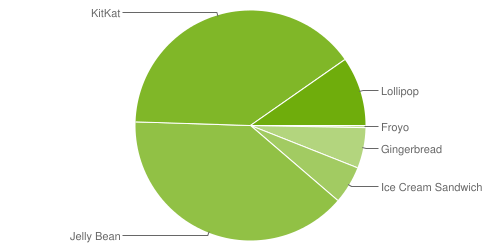
\includegraphics[keepaspectratio, scale=0.8]{Media/Captures/androidUsage.png}
      \caption{Distribución Actual de Versiones Android (Fuente: Google)}
      \label{fig:android_Usage}
    \end{figure}
	
	
    
    \subsection{XML}\label{ssec:xml}
    
	XML \cite{ref:xml} (eXtensible Markup Language) es un formato de definición, almacenamiento e intercambio de datos de forma estructurada. Fue definido en 1996 por el W3C y actualmente existe una versión 1.1 (2008). Se trata de un lenguaje de marcado que define dicho formato estructurado mediante marcas o ''etiquetas'' que aportan información acerca del texto que rodean. En el caso particular de Android, esta plataforma define la interfaz gráfica de sus pantallas mediante documentos XML llamados Layouts \cite{ref:android_layout}.
	
	En este proyecto se utilizará XML para definir la interfaz gráfica de las pantallas que conforman la aplicación Android. 
    
    \subsection{JSON}\label{ssec:json}
    
	JSON \cite{ref:json} (JavaScript Object Notation) es un estándar para intercambio de datos de forma simple y ligera mediante pares clave-valor. Originalmente derivaba de un subconjunto de datos de JavaScript pero actualmente se encuentra definido en el RFC 7159 y el ECMA-404 y es independiente de lenguaje que se utilice para interpretar (''parsear'') los datos que contiene. En JSON se puede estructurar estos datos de dos formas: en objetos (que contienen pares clave-valor) y en arrays (que contienen objetos).
	
	En este proyecto utilizaremos JSON para intercambiar datos con el servidor de Wave/SwellRT y con el Service REST de la aplicación. En el caso de SwellRT no trabajaremos directamente a nivel de JSON ya que su API abstrae el formato de intercambio de datos. Sin embargo, en la aplicaión sí que trabajaremos directamente con esta tecnología ya que el Service REST responde a las peticiones de la aplicación en forma de mensajes JSON que la propia aplicación debe tambien ''parsear'' para tratarlos.    
    
    \subsection{SQL}\label{ssec:sql}
    
	SQL \cite{ref:sql} (Structured Query Language) es un lenguaje diseñado específicamente para interactuar con Bases de Datos Relacionales pudiendo definir la estructura de los datos y manipularlos. Desarrollado en 1986, actualmente está estandarizado por la International Standards Organization (ISO) en el estándar ISO/IEC 9075 SQL \cite{ref:sql}. Este lenguaje permite mediante la construcción de ''consultas'' crear tablas, acceder a sus datos y modificarlos entre otras cosas.
	
	En este proyecto se utilizará SQL en el Service REST para construir las consultas a Base de Datos necesarias para devolver al cliente de la aplicación Android los datos que solicite o pida cambiar.  
    
    \subsection{MySQL}\label{ssec:mysql}
    
	MySQL \cite{ref:mysql} es un Sistema Gestor de Base de Datos (SGBD) Relacionales que permite el almacenamiento, creación y modificación de dicho tipo de Bases de Datos. Desarrollado por Oracle, su versión actual (5.7.4) se distribuye tanto en forma de Software libre (bajo licencia GPL) o de uso comercial.     
	
	En este proyecto se usará MySQL como SGBD para almacenar la Base de Datos de nuestra aplicaión Android.
    
    \subsection{PhpMyAdmin}\label{ssec:phpmyadmin}
    
	PhpMyAdmin \cite{ref:phpMyAdmin} es una herramienta de código libre (bajo licencia pública GNU) escrita en PHP y que proporciona un sistema de administración de SGBD MysQL a través de una interfaz web. Fue desarrollado en 1998 y actualmente la versión 4.4.8 es desarrollada y mantenida por The PhpMyAdmin Project. Posee una interfaz sencilla que permite administrar la Base de Datos mediante las operaciones básicas de creación, modificación, eliminación de tablas,  creación de consultas SQL y gestión de permisos y usuarios entre otros.
	
	En este proyecto se usará PhpMyAdmin como sistema de administración de la Base de Datos MySQL que contiene los datos de la aplicación Android.
    
    \subsection{PHP}\label{ssec:php}
    
	PHP \cite{ref:php} es un lenguaje de propósito general del lado del servidor diseñado originalmente para crear aplicaciones web que generaran contenido dinámico. Diseñado en 1996 por Rasmus Lerdorf, su versión actual 5.6.7 es de código libre y se distribuye bajo licencia PHP. Tiene la ventaja de poder ser fácilmente incorporado dentro de los documentos HTML.
	
	Para este proyecto se utilizará el lenguaje PHP para programar el comportamiento del Service REST que hace de intermediario entre las peticiones de la aplicación Android y la Base de Datos MySQL.
    
    \subsection{Laravel 5}\label{ssec:laravel}
    
	Laravel \cite{ref:laravel} es un framework que permite desarrollar aplicaciones y servicios web con PHP 5. Fue desarrollado por Taylor Otwell en 2011 y su versión actual 5.0 se distribuye en forma de código abierto (bajo licencia MIT) en su propio repositorio público en GitHub \cite{ref:laravel_github}. Su funcionalidad es extensible mediante módulos.
	
	En este proyecto se utilizará Laravel 5 para construir en PHP el Service REST que hará de intermediario entre las peticiones HTTP del cliente Android y la Base de Datos de la aplicación.
	
	La elección de Laravel como framework PHP se debió a su flexibilidad, la facilidad para programar la aplicación y el gran soporte que tiene de la comunidad. Además, es uno de los frameworks más populares actualmente en uso.
	
\begin{figure}[!]
\centering
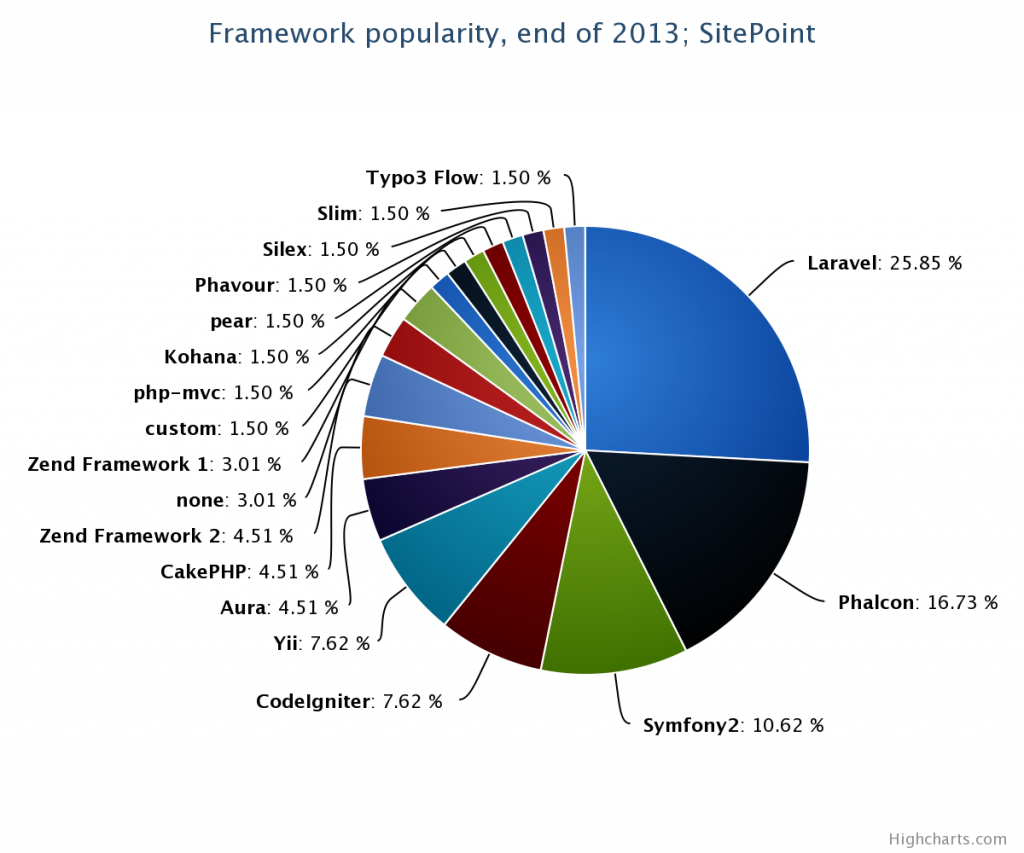
\includegraphics[keepaspectratio, scale=0.30]{Media/Captures/frameworkPopularity.png}
\caption{Frameworks PHP más populares. Fuente: SitePoint}
\label{fig:laravel5popularity}
\end{figure}
    
    \subsection{OpenShift}\label{ssec:openshift}
    
	OpenShift \cite{ref:OpenShift} es una plataforma de computación en la nube que ofrece alojar servicios de forma gratuita en sus servidores mediante un modelo de arquitectura Software as a Service (SaaS). Disponible desde 2011, se distribuye bajo licencia Apache 2.0. Dispone también de planes de pago que aumentan las prestaciones del servidor.
	
	En este proyecto se usará OpenShift como servidor web para alojar los servicios de los que hace uso nuestra aplicación Android: el Servicio Web REST y la Base de Datos. Concretamente el servidor esta accesible desde la siguiente URL:
	
	\url{HTTPs://apptfg-servicerest.rhcloud.com/}    
    
    \subsection{Sublime Text}\label{ssec:sublime}
    
    Sublime Text \cite{ref:sublime} es un editor de texto gratuito multiplataforma muy versátil que proporciona características de atajos de teclado y resaltado de código para diferentes lenguajes de programación muy útiles cuando se desarrolla sin un IDE. Fue desarrollado en 2008 por Jon Skinner y actualmente se encuentra en su versión 2.0.2.
    
    En este proyecto se utilizará Sublime como editor de texto sobre todo para configurar y programar el Service REST en PHP, pues no se ve necesario utilizar un IDE específico para ello.
    
    \subsection{POP: Prototyping On Paper}\label{ssec:pop}
    
    POP \cite{ref:pop} (Prototyping On Paper) es una aplicación con versiones web y para dispositivos móviles que permite elaborar en pocos pasos prototipos (mockups) interactivos basados en fotos de prototipos realizados en papel. De esta forma se puede elaborar un prototipo de interfaz gráfica de bajo coste con la que el usuario pueda interactuar.
    
    Ene este proyecto se utilizará POP durante la fase de diseño de la aplicación Android para elaborar mockups sencillos e interactivos que podamos enseñar a la gente y que nos ayuden a refinar el diseño de la interfaz gráfica de la aplicación. Tiene además la ventaja de que se puede enseñar en la aplicación móvil de POP para simular el aspecto final que tendría la aplicación y que el usuario se haga una mejor idea de lo que se pretende diseñar.
    